\subsection{Run Time View}

This section provides a detailed perspective on how the system internally works and its component interact with each other at runtime. It focuses on the dynamic aspects of the software, emphasizing the flow of control, data, and communication between different modules or components.\newline
Just as a note, in order to make the diagrams more readable, some abbreviations have been used in the methods exposed by the various interfaces of \app components (as shown in section 2.5). In particular, tournamentName is tName, battleName is bName.


\subsubsection*{Educator login}
\begin{figure}[h!]
    \centering
    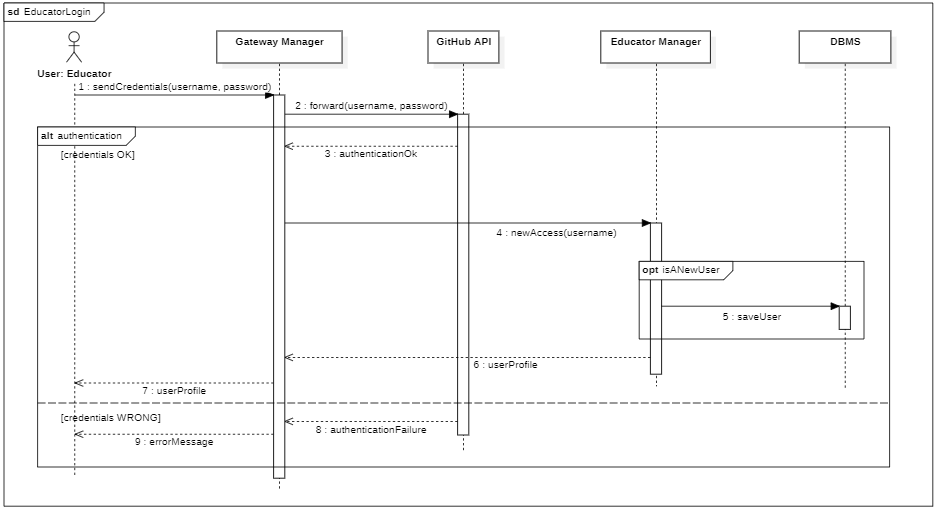
\includegraphics[width=1\linewidth]{1Sequence_EducatorLogIn}
    \caption{Runtime view of the login of an educator}
    \label{fig:educator_login}
\end{figure}

The educator login process unfolds in the following manner: the Educator initiates the login by contacting the Gateway Manager and transmitting their credentials. Subsequently, the Gateway Manager interfaces with the GitHub API to verify and authorize access. Two possible scenarios may unfold: a successful authentication or an unsuccessful one. In the latter case, an error message is generated and displayed to the Educator. In the event of a successful authentication, the Gateway Manager communicates with the Educator Manager, forwarding all relevant data to be stored in case it is the Educator's first sign-in. In both scenarios, the Educator Manager is responsible for returning the user profile to the Educator.

This process ensures a seamless and secure login experience, with appropriate feedback provided to the Educator based on the outcome of the authentication process.
\newpage

\subsubsection*{Student login}
\begin{figure}[h!]
    \centering
    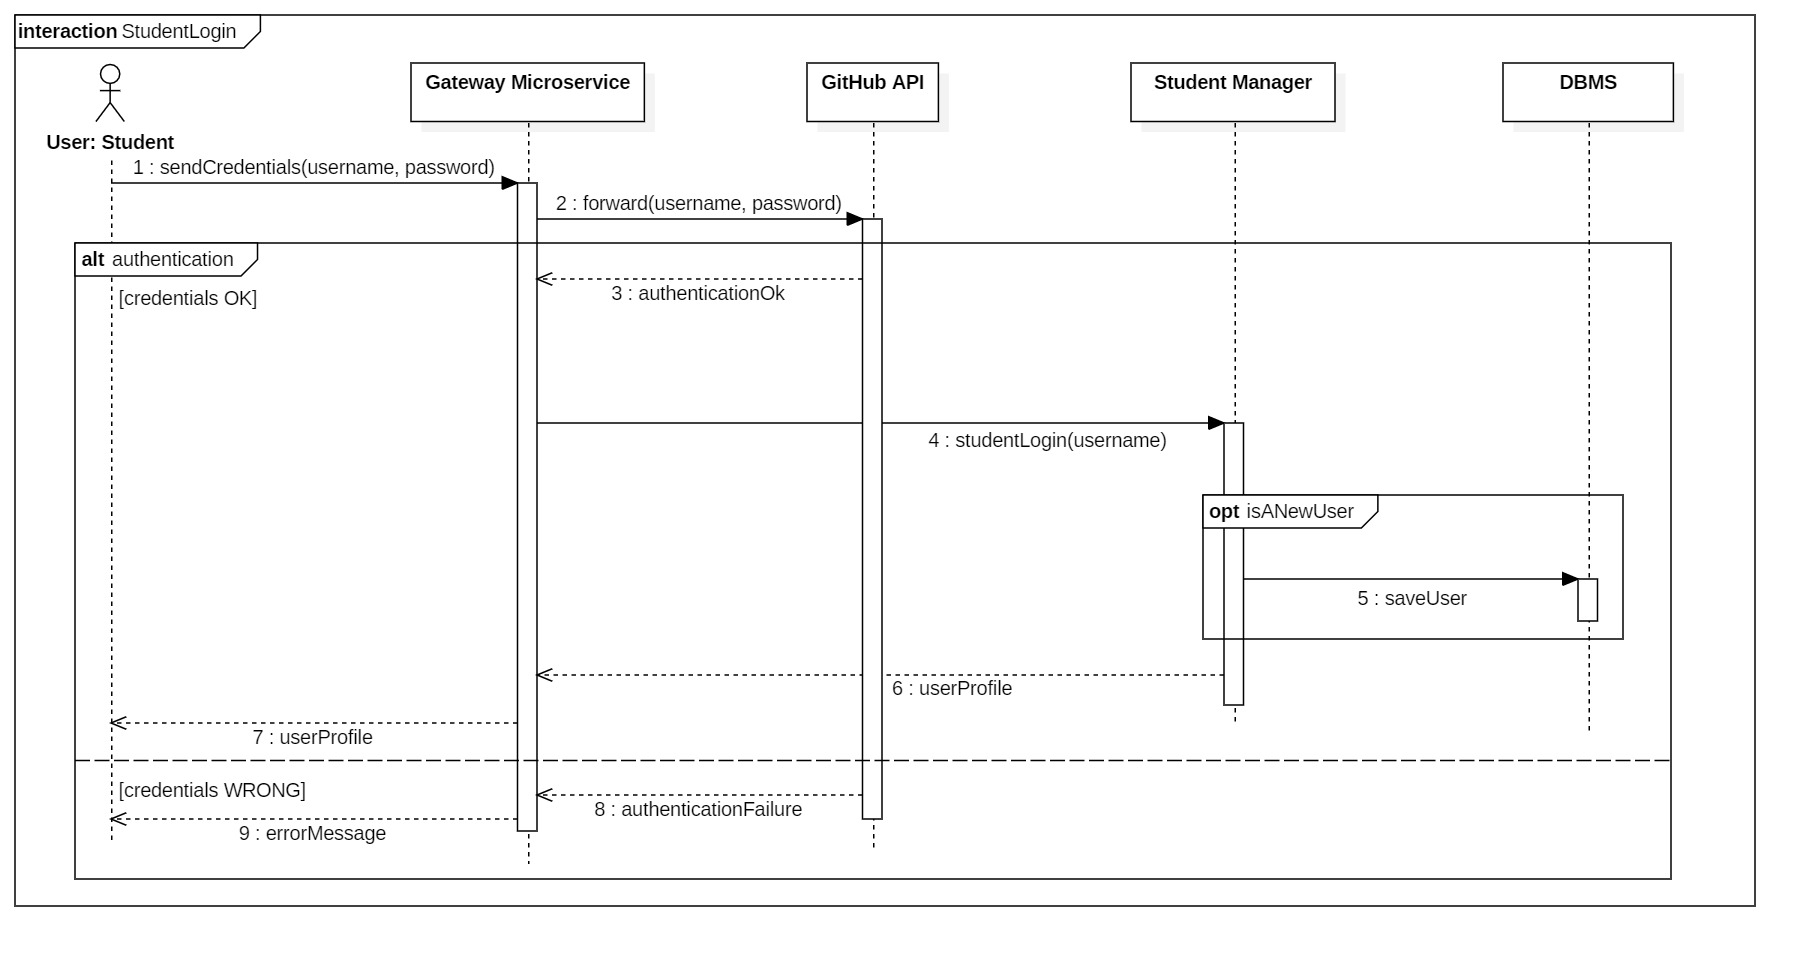
\includegraphics[width=1\linewidth]{2.ArchitecturalDesign/res/StudentLogin.jpg}
    \caption{Runtime view of the login of a student}
    \label{fig:student_login}
\end{figure}

The student login process mirrors that of the educator, with the primary distinction lying in the actor, now the student, and the involvement of different microservices. Here's how it unfolds: the Student initiates the login process by reaching out to the Gateway Manager and submitting their credentials. Subsequently, the Gateway Manager interfaces with the GitHub API to validate and authorize access.

Similar to the educator's login process, two potential outcomes are possible: a successful authentication or an unsuccessful one. In the case of an unsuccessful authentication, an error message is generated and presented to the student. However, in the event of a successful authentication, the Gateway Manager now communicates directly with the Student Manager. The Student Manager is then responsible for handling the data, including storage in the case of the student's initial sign-in, and returning the user profile to the student.

Despite the differences in actors and microservices, the student login process ensures a comparable and secure user experience, tailored to the specific needs of the student user role.

\newpage

\subsubsection*{Tournament creation}
\begin{figure}[h!]
    \centering
    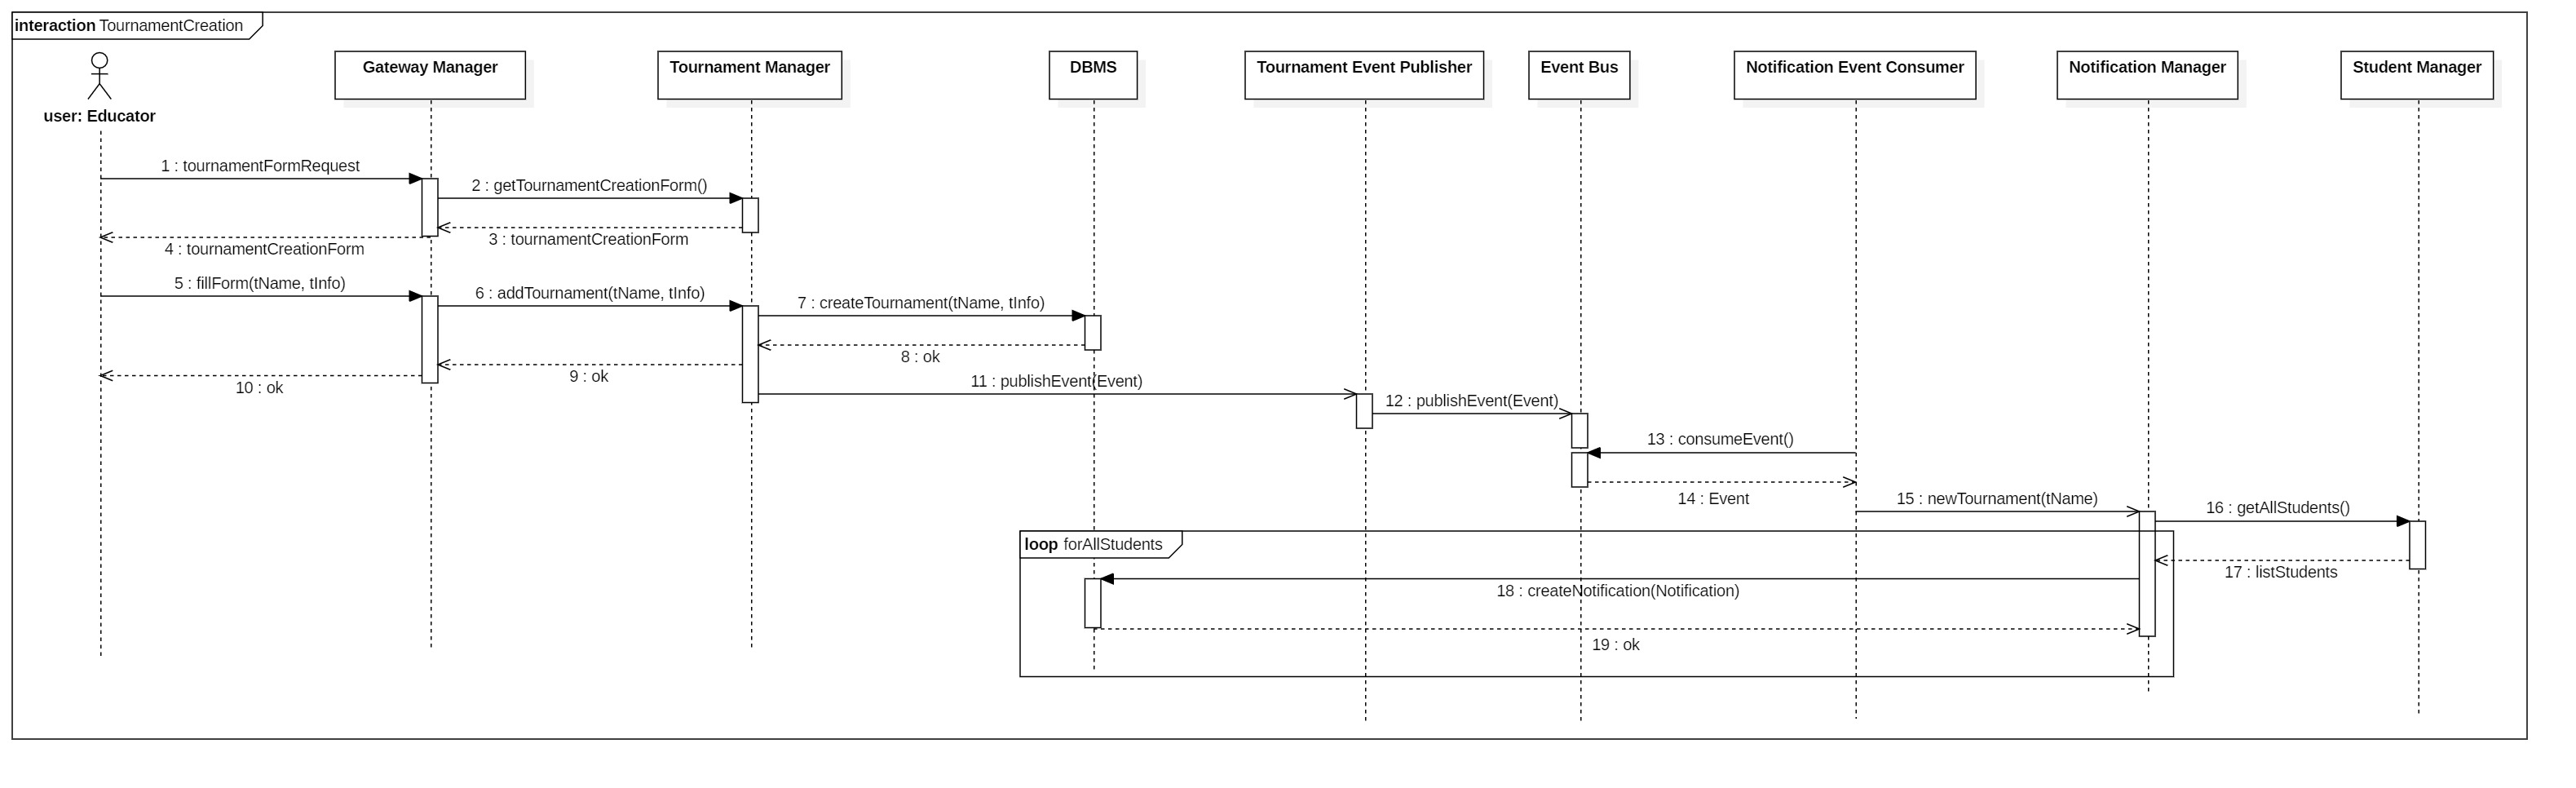
\includegraphics[width=1.3\linewidth, angle=90]{2.ArchitecturalDesign/res/TournamentCreation.jpg}
    \caption{Runtime view of the creation of a tournament}
    \label{fig:tournament_creation}
\end{figure}

In Figure \ref{fig:tournament_creation}, the diagram illustrates the interactions between components when an educator initiates the creation of a new tournament. Initially, the educator contacts the Gateway Manager, which then sends a request to the Tournament Manager in order to obtain the form necessary for the creation process. After receiving the form, the educator fills it out and sends it back to the Tournament Manager. The Tournament Manager stores the information in the DBMS and triggers a notification to signify the successful creation of the tournament. 

While the specific details of this notification process will be discussed momentarily, it is worth noting that this sequence remains consistent across various runtime views and will be omitted in subsequent descriptions.

Subsequently, the Tournament Publisher receives the data pertaining to the newly created tournament and communicates with the Event Bus to publish this information. Then, asynchronously, the Notification Consumer polls the Event Bus, retrieving the new event. Once obtained, the Notification Consumer generates a notification and forwards it to the Student Manager. The Student Manager then iterates through all the students, ensuring each receives the notification.

\newpage

\subsubsection*{Battle creation}
\begin{figure}[h!]
    \centering
    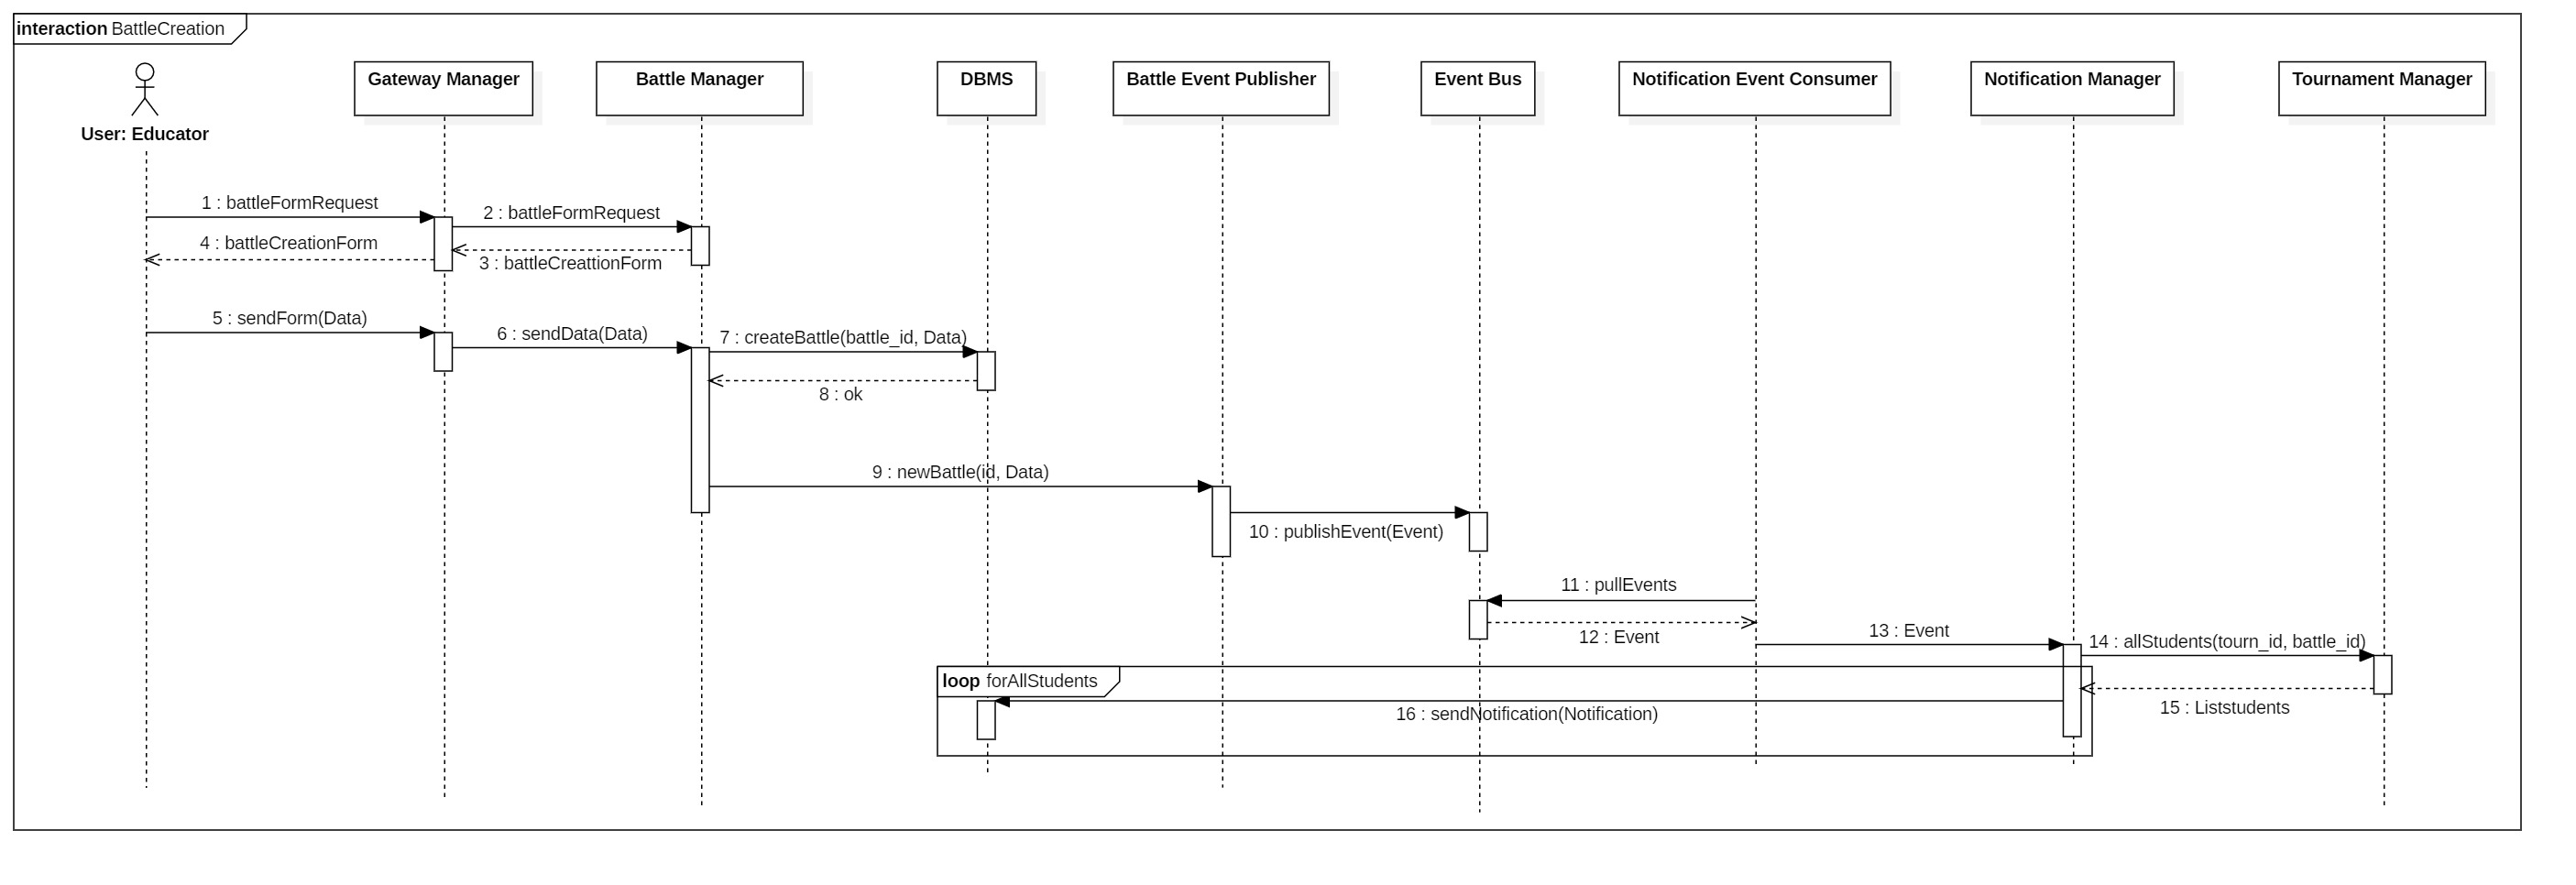
\includegraphics[width=1.3\linewidth, angle=90]{2.ArchitecturalDesign/res/BattleCreation.jpg}
    \caption{Runtime view of the creation of a battle}
    \label{fig:battle_creation}
\end{figure}

The process for battle creation mirrors that of tournaments. The Educator initiates the process by sending a request to the Gateway Manager, which forwards the request to the Battle Manager. The Battle Manager responds by providing the necessary form for the Educator to complete. Subsequently, the Educator fills out the form and returns it to the Battle Manager. The Battle Manager then stores the information for the newly created battle in the DBMS. Similar to the tournament creation, a new event is generated.

It's important to note that, in this context, all the students notified will only be those subscribed to the tournament in which the battle has been created.

\newpage

\subsubsection*{End of a tournament}
\begin{figure}[h!]
    \centering
    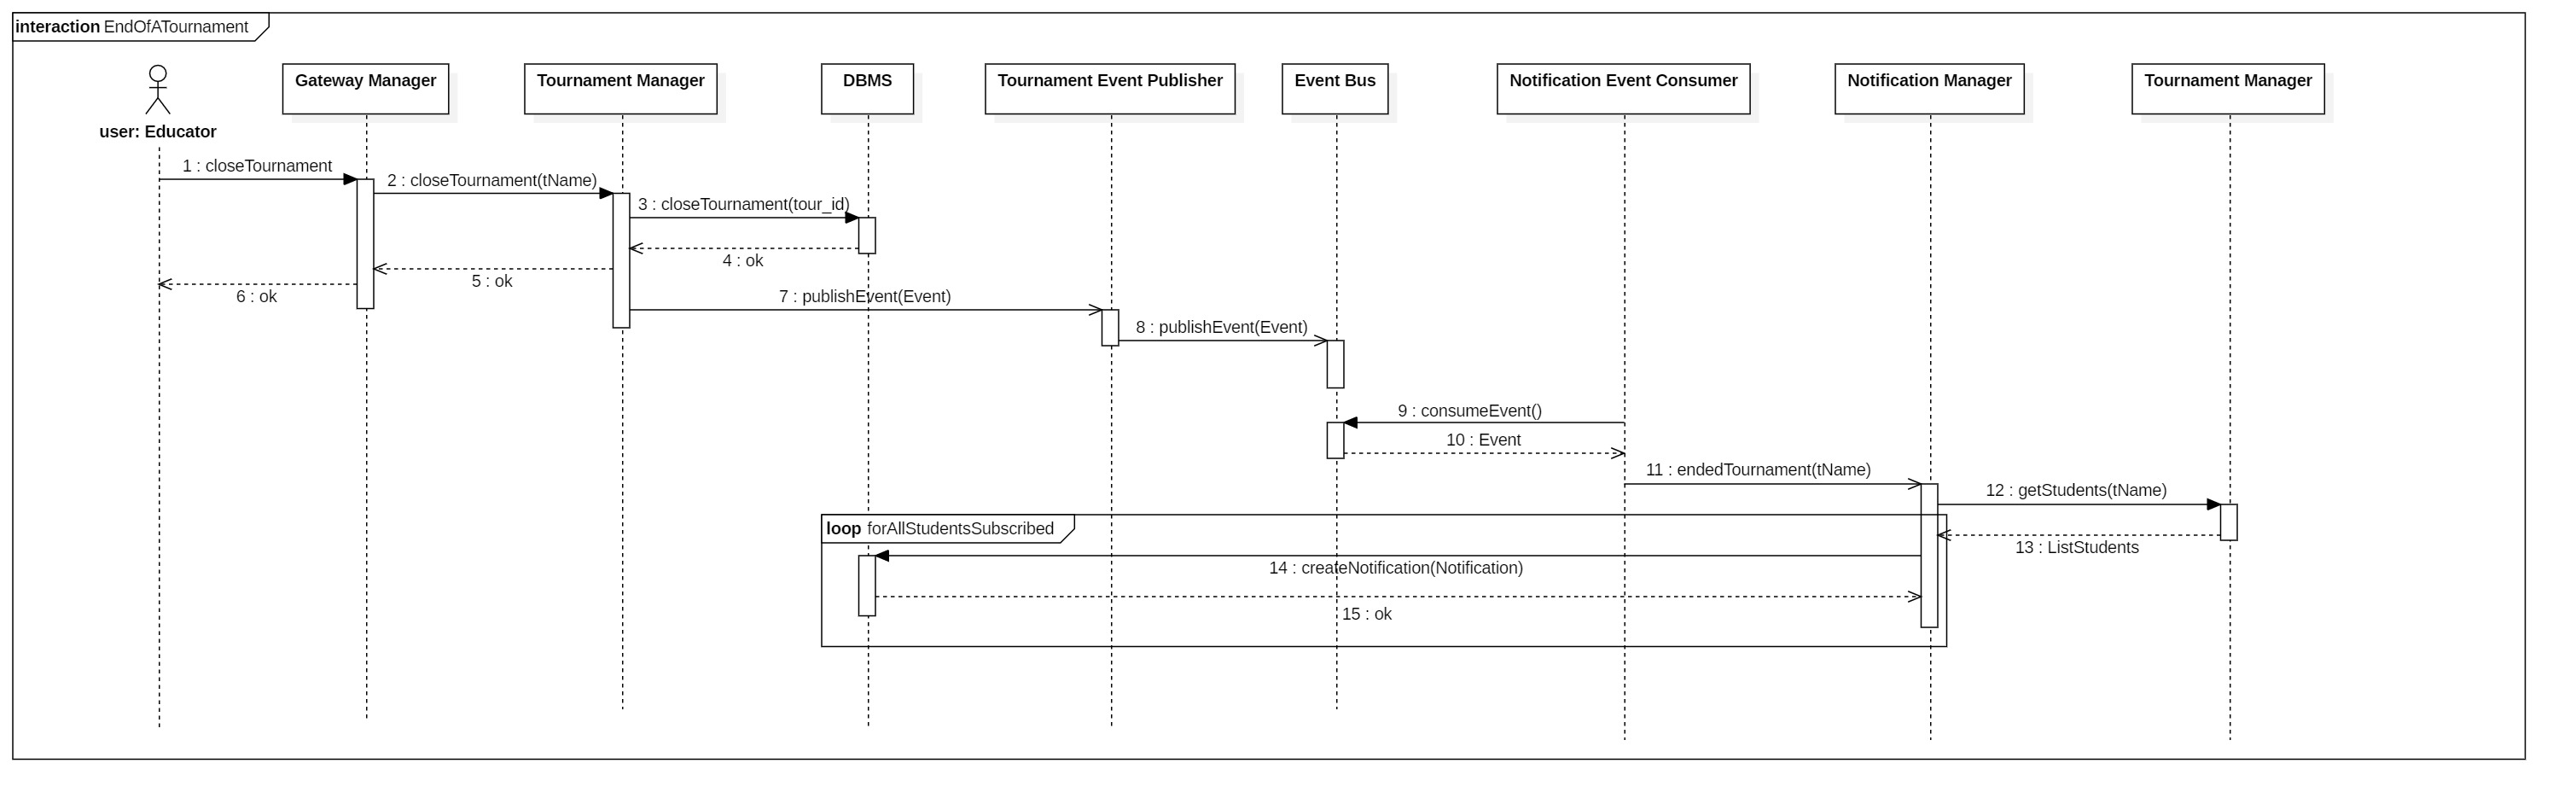
\includegraphics[width=1.3\linewidth, angle=90]{2.ArchitecturalDesign/res/EndOfATournament.jpg}
    \caption{Runtime view when the end of a tournament is reached}
    \label{fig:tournament_end}
\end{figure}

When a tournament concludes, the determination is made by the Educator, who initiates the process by sending a request to the Gateway Manager. The Gateway Manager then forwards this request to the Tournament Manager, which in turn updates the relevant data regarding the tournament in the DBMS. Following the update, a new event is generated and disseminated to all the students who have subscribed to that particular tournament, adhering to the previously outlined notification mechanism.

\newpage

\subsubsection*{End of a battle}
\begin{figure}[h!]
    \centering
    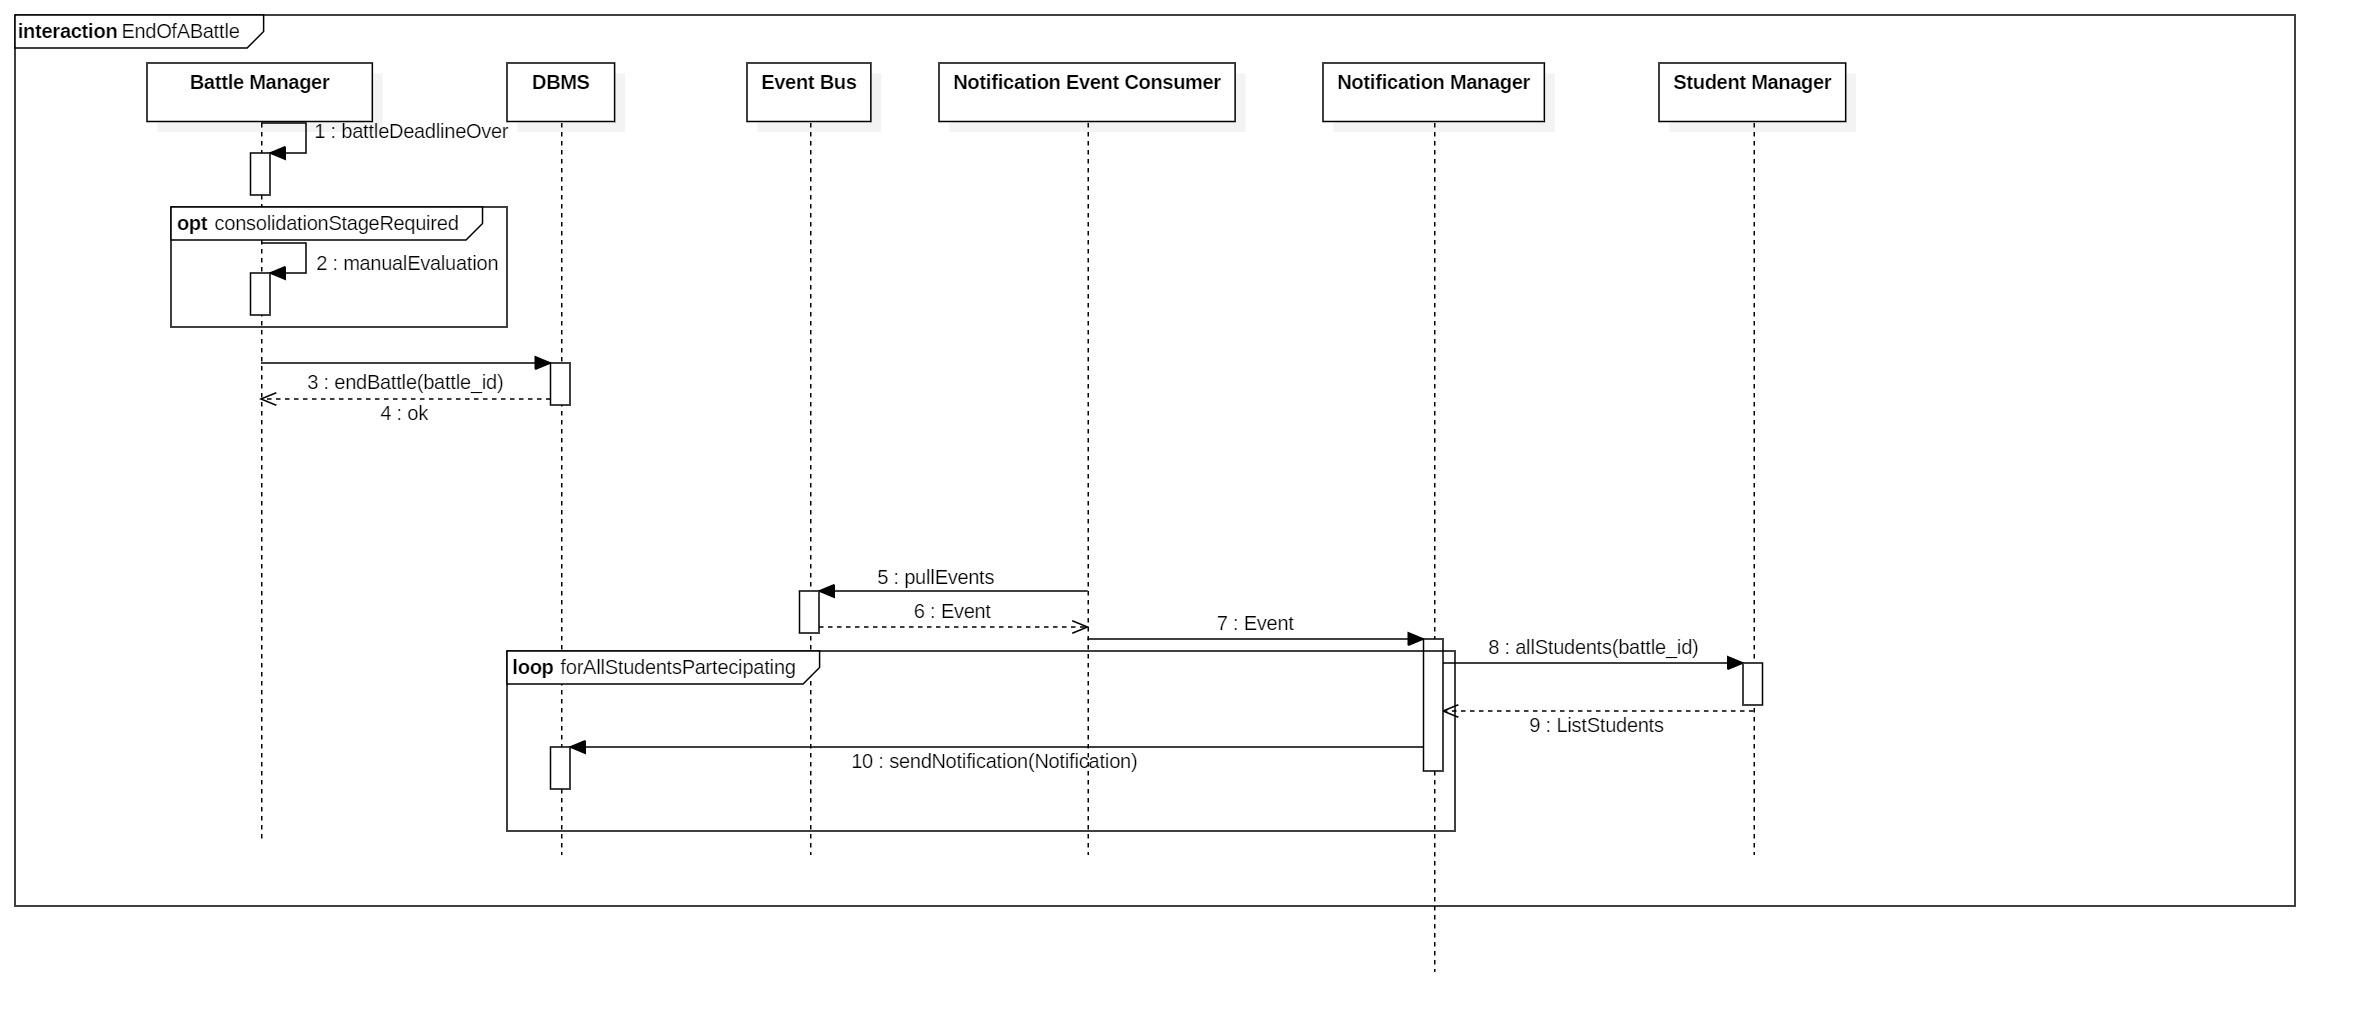
\includegraphics[width=1.3\linewidth, angle=90]{2.ArchitecturalDesign/res/EndOfABattle.jpg}
    \caption{Runtime view when a battle ends}
    \label{fig:battle_end}
\end{figure}

The conclusion of a battle occurs upon reaching its specified deadline, and the mechanism for monitoring this may involve a polling system, depending on the chosen development framework. Once the deadline is reached, the system checks whether a manual evaluation is required, as determined during the battle's creation. Subsequently, the parameters of the battle are updated by interacting with the DBMS. Following this update, an event is generated, mirroring the previously described process, and disseminated accordingly.

\newpage

\subsubsection*{Subscribe To Tournament}
\begin{figure}[h!]
    \centering
    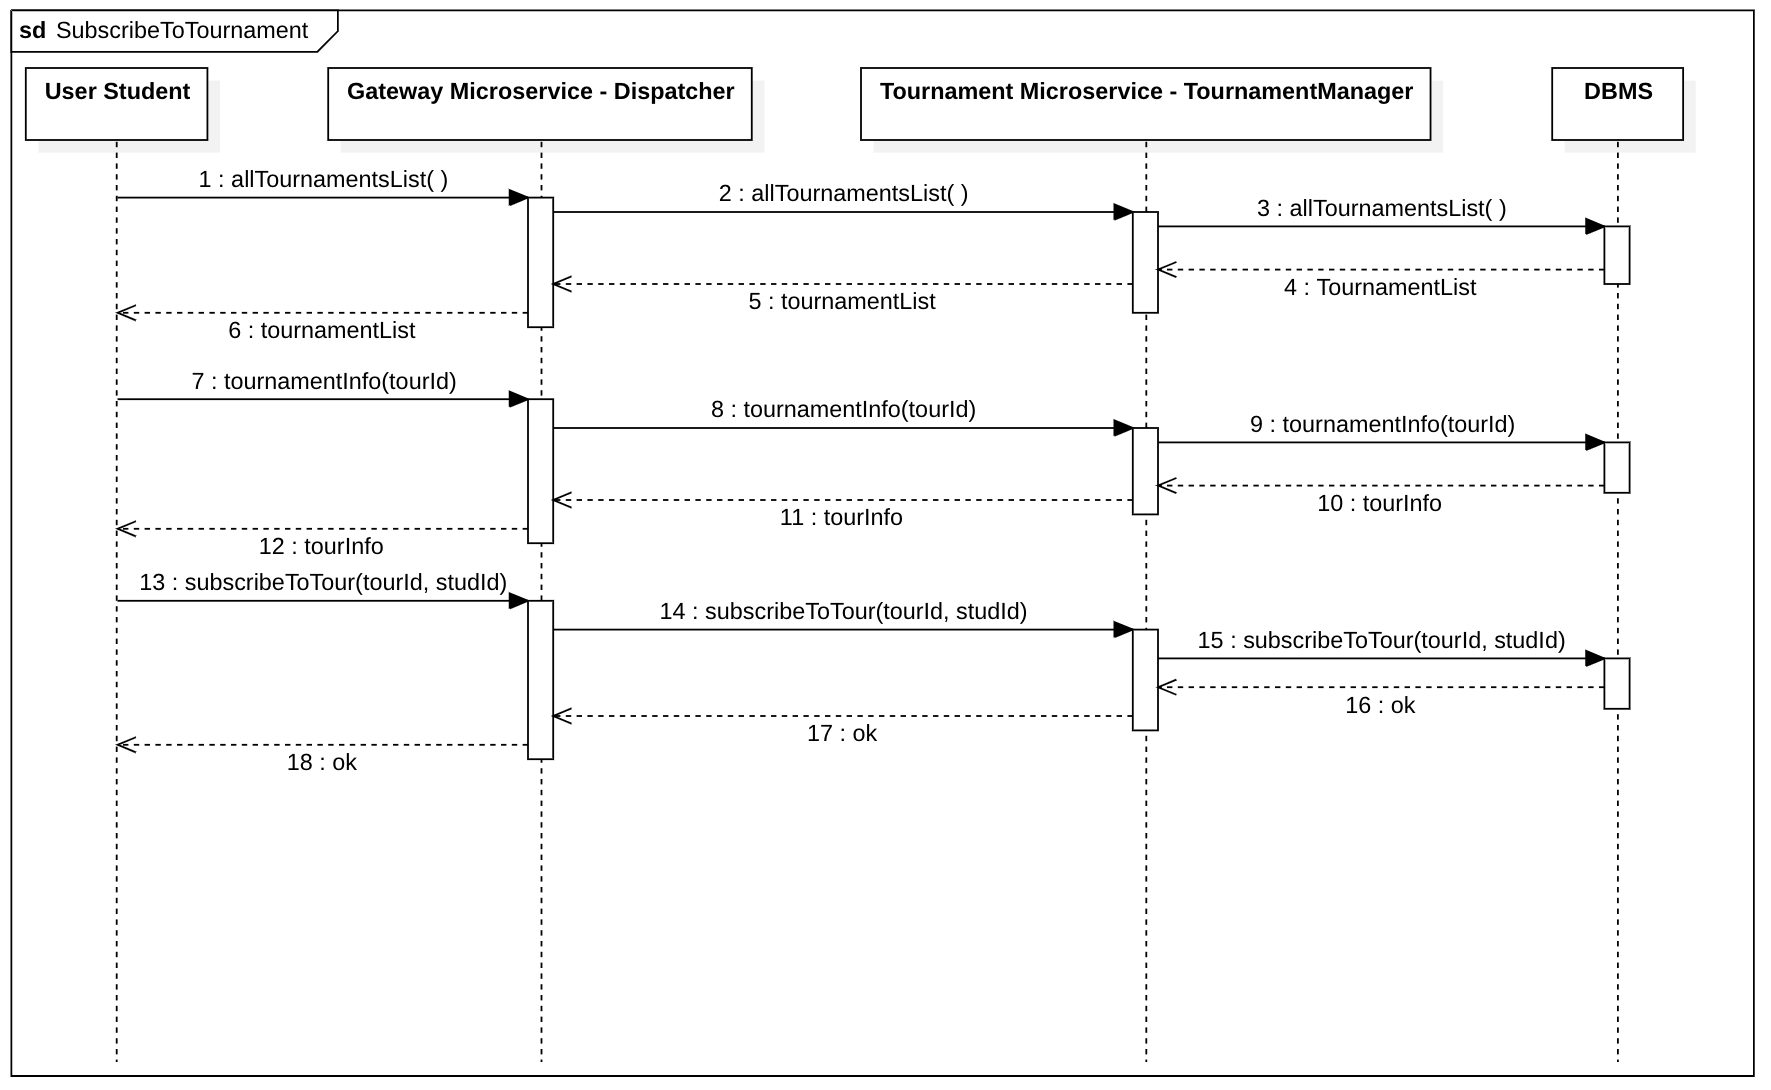
\includegraphics[width=1\linewidth]{2.ArchitecturalDesign/res/subscribeToTournament.jpg}
    \caption{Runtime view when a student subscribes to a tournament}
    \label{fig:subsTournament}
\end{figure}

The client initiates a request for a list of tournaments. This request is transmitted to the gateway component, which acts as an intermediary.
The gateway, upon receiving the request, forwards it to the Tournament Manager microservice. The Tournament Manager retrieves the relevant information from the database and subsequently transmits the data back to the gateway.
The gateway, in turn, relays the tournament list to the client.\\
Subsequently, the client initiates a request for specific information about a particular tournament. This request traverses the gateway before reaching the Tournament Manager microservice. The Tournament Manager retrieves the requisite details from the Database Management System (DBMS) and transmits the information back.\\
Lastly, the client issues a subscription request. This request is routed through the gateway to the Tournament Manager. The Tournament Manager processes the request by writing the new subscription details to the DBMS, thereby completing the subscription process. After the processs is completed a confirmation message is trasmitted back.

\newpage

\subsubsection*{Subscribe To Battle}
\begin{figure}[h!]
    \centering
    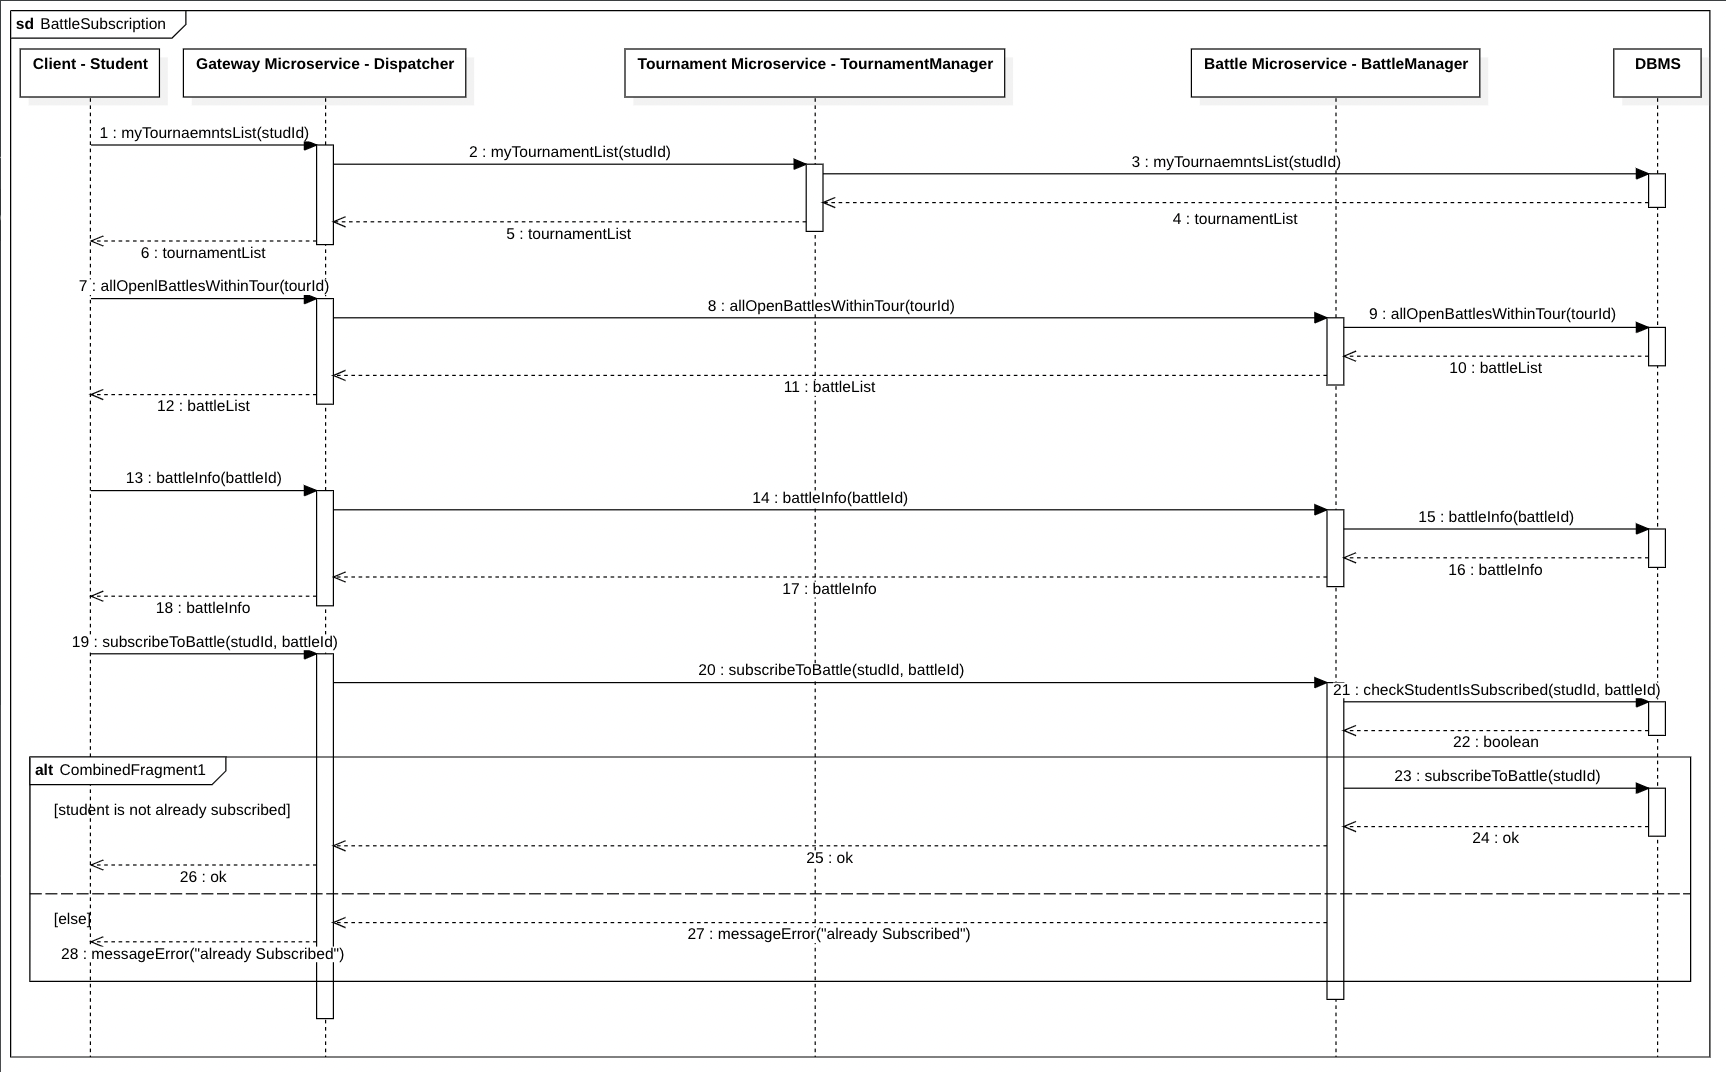
\includegraphics[width=1.3\linewidth, angle=90]{2.ArchitecturalDesign/res/subscribeToBattle.png}
    \caption{Runtime view when a student subscribes to a battle}
    \label{fig:subsBattle}
\end{figure}

The sequence begins with the client initiating a request for the list of tournaments. This request is directed to the gateway component.
The gateway, acting as an intermediary, forwards the tournament list request to the Tournament Manager microservice. The Tournament Manager retrieves the pertinent information from the Database Management System (DBMS) and transmits it back to the gateway.
Subsequently, the gateway relays the tournament list to the client.\\
Following this, the client makes a request for the list of battles within a specific tournament, specifically those currently open for subscription. This request is initially routed through the gateway before being further directed to the Battle Manager microservice.
The Battle Manager, upon receiving the request, retrieves the relevant information from the database and sends the list of open battles back through the gateway to the client.\\
Subsequently, the client sends a subscription request for a specific battle. The subscription request first traverses the gateway and then reaches the Battle Microservice.
Within the Battle Microservice, the system checks the database to verify if the student is already subscribed to the specified battle. If the student is already subscribed, an error message is generated and transmitted back to the client.
If the student is not already subscribed, the Battle Manager writes the new subscription details to the database and generates a confirmation of the subscription.
The confirmation of the subscription is then sent back through the gateway to the client.

\newpage

\subsubsection*{Educator Gives Permission}
\begin{figure}[h!]
    \centering
    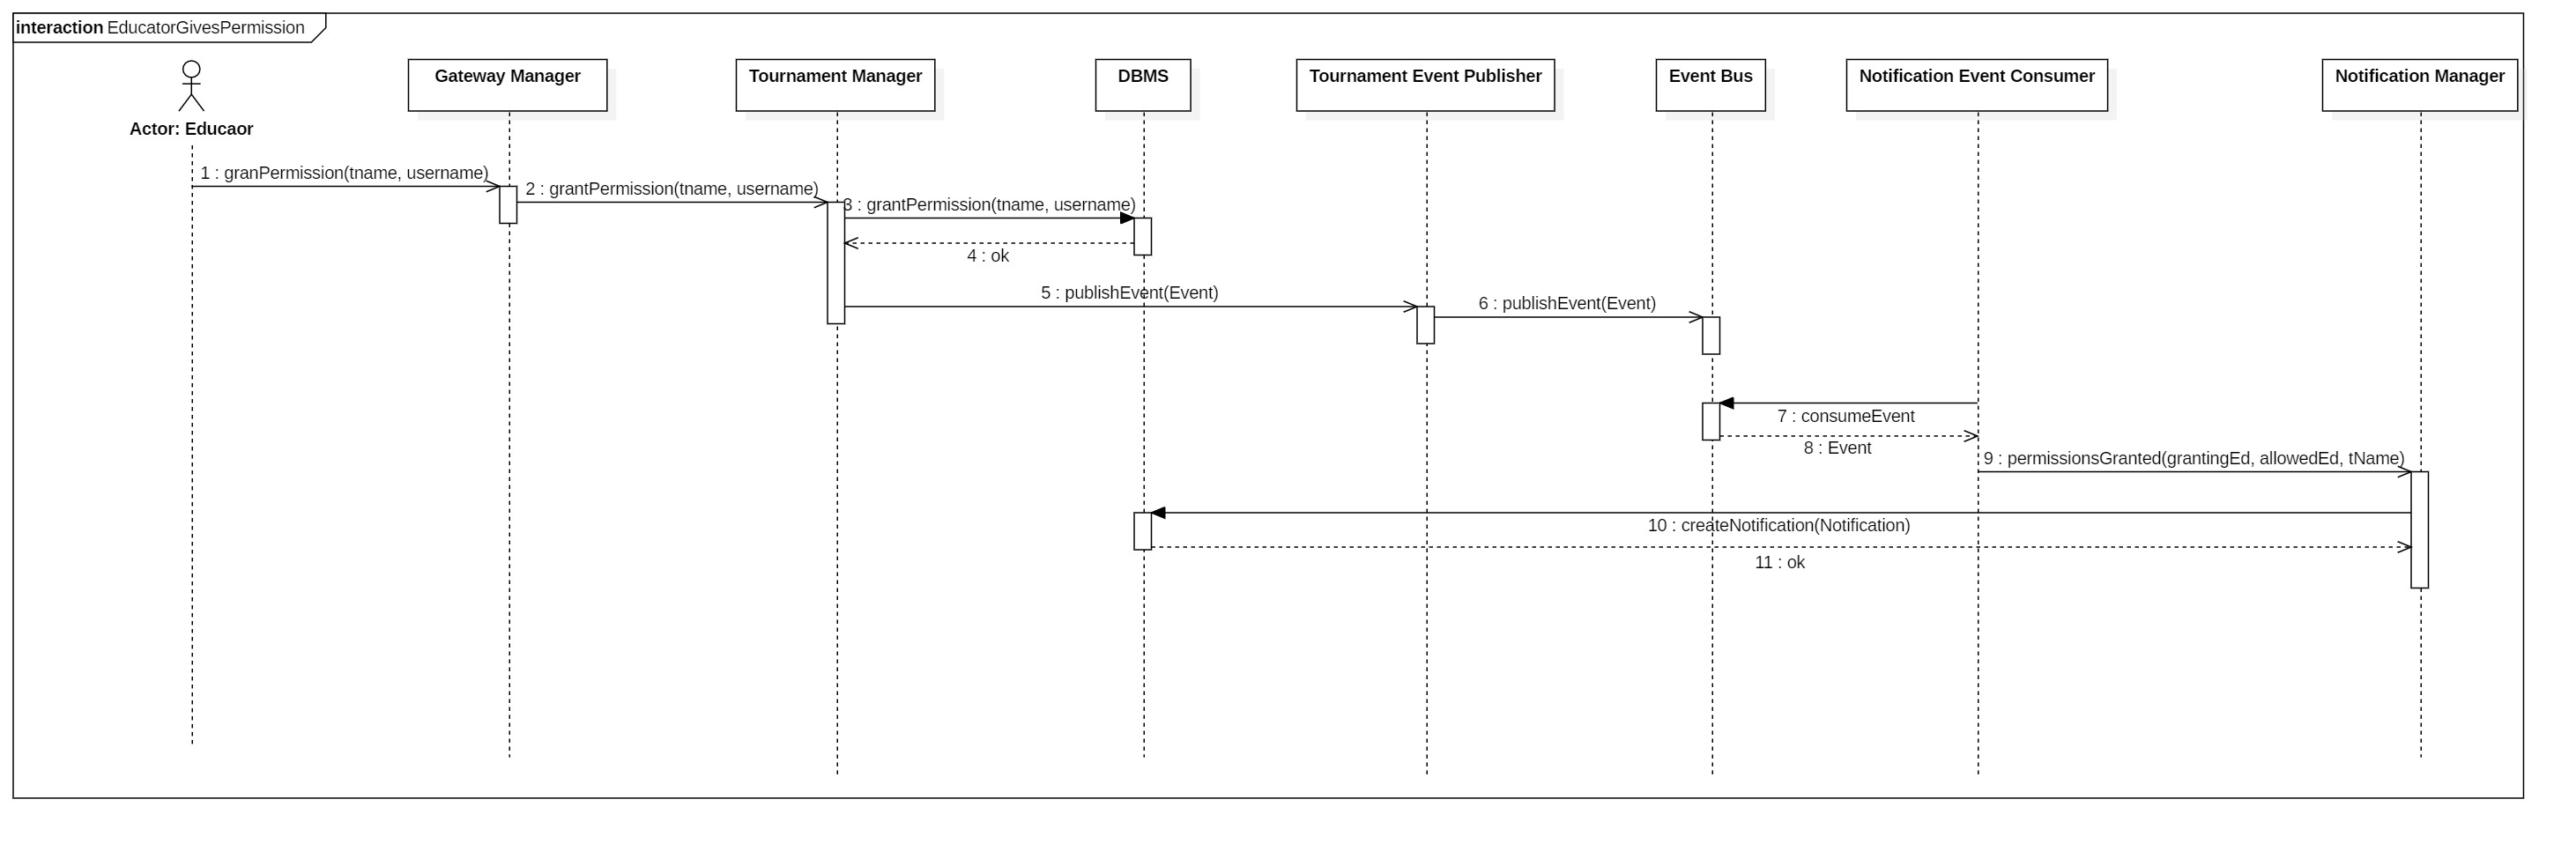
\includegraphics[width=1.3\linewidth, angle=90]{2.ArchitecturalDesign/res/EducatorGivesPermission.jpg}
    \caption{Runtime view of the educator giving permission to another one for a tournament he owns}
    \label{fig:permission}
\end{figure}

The sequence starts with the Educator engaging with the Gateway Manager to request the possibility of grant permission for a tournament they own. To do this, the Educator sends a request that includes the tournament name and their username for identification.
The Gateway Manager then redirects the request to the appropriate component, the Tournament Manager, which saves the new information in the Database by interacting with the DBMS, receiving then an affirmative response.
After completing this step, the Tournament Manager must generate a new Notification. As mentioned earlier, the Publisher publishes the new Event to the Event Bus, and the Notification Event Consumer, in collaboration with the Notification Manager, creates the new Notification, saving it into the Database with the assistance of the DBMS component.

\newpage

\subsubsection*{Badge Assignment}
\begin{figure}[h!]
    \centering
    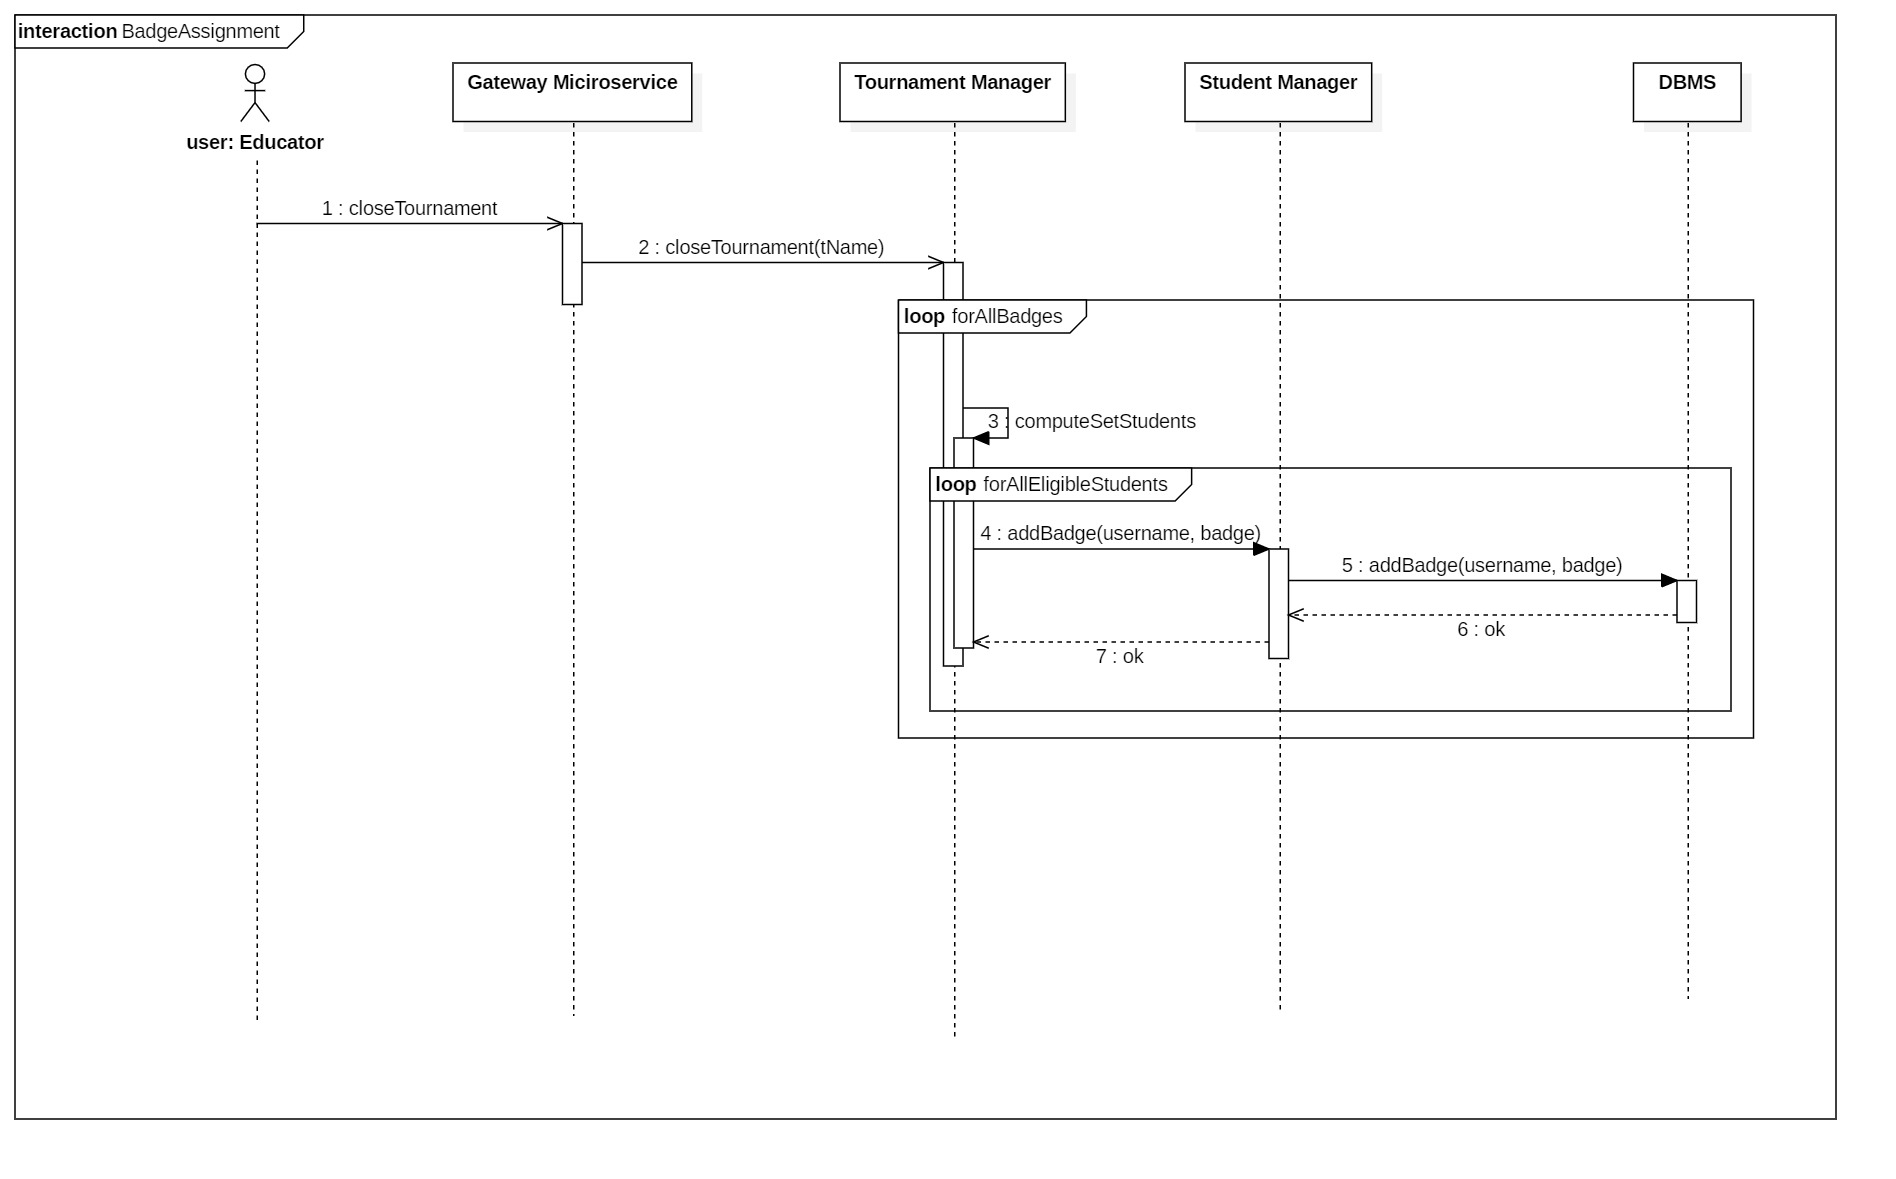
\includegraphics[width=1.3\linewidth, angle=90]{2.ArchitecturalDesign/res/BadgeAssignment.jpg}
    \caption{Runtime view of the assignment of badges}
    \label{fig:badge}
\end{figure}

The sequence starts with the closure of a tournament (see Figure \ref{fig:tournament_end}). Following the closure, the Tournament Manager calculates all the badges to be assigned to the respective teams and, consequently, to the individual students. The loop in the diagram illustrates the process of sending these badges and saving the corresponding data in the DBMS by the Student Manager.

\newpage

\subsubsection*{Code Push}
\begin{figure}[h!]
    \centering
    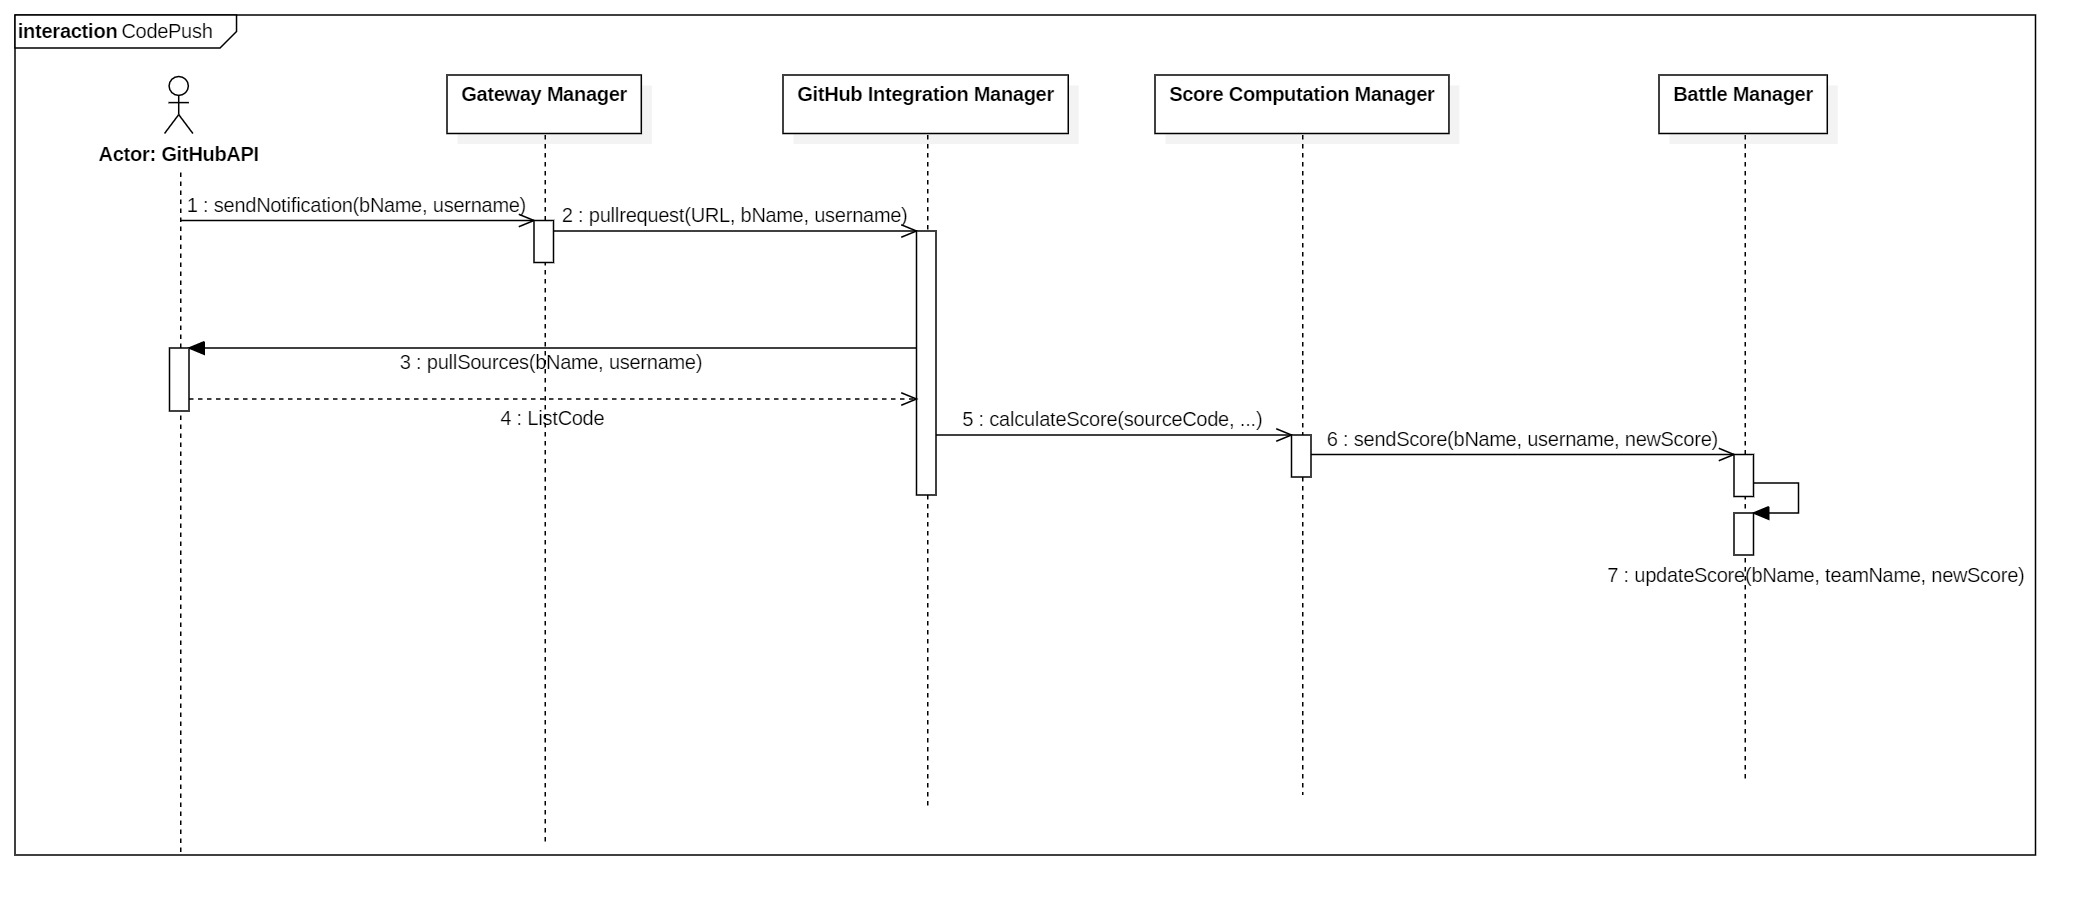
\includegraphics[width=1.3\linewidth, angle=90]{2.ArchitecturalDesign/res/CodePush.jpg}
    \caption{Runtime view when a student pushes the code}
    \label{fig:push}
\end{figure}

The process begins with the action of pushing code, initiated by receiving a notification from the GitHub API indicating that code has been pushed. This notification is received by the Gateway Manager, which then contacts the GitHub Integration Manager to request a pull of the code. The method parameters include the repository URL, the battle name, and the student's username who pushed the code.
Subsequently, the GitHub Integration Manager requests the GitHub API to pull the source code, resulting in a list of code documents that are essential for calculating scores. Following this, the GitHub Integration Manager asks the Score Computation Manager to compute scores, considering various factors such as source code quality, build scripts, test cases, elapsed time, and evaluation criteria.
After calculating the scores, the Score Computation Manager sends the results to the Battle Manager, which updates the local scores accordingly.

\newpage

\subsubsection*{Repository creation}
\begin{figure}[h!]
    \centering
    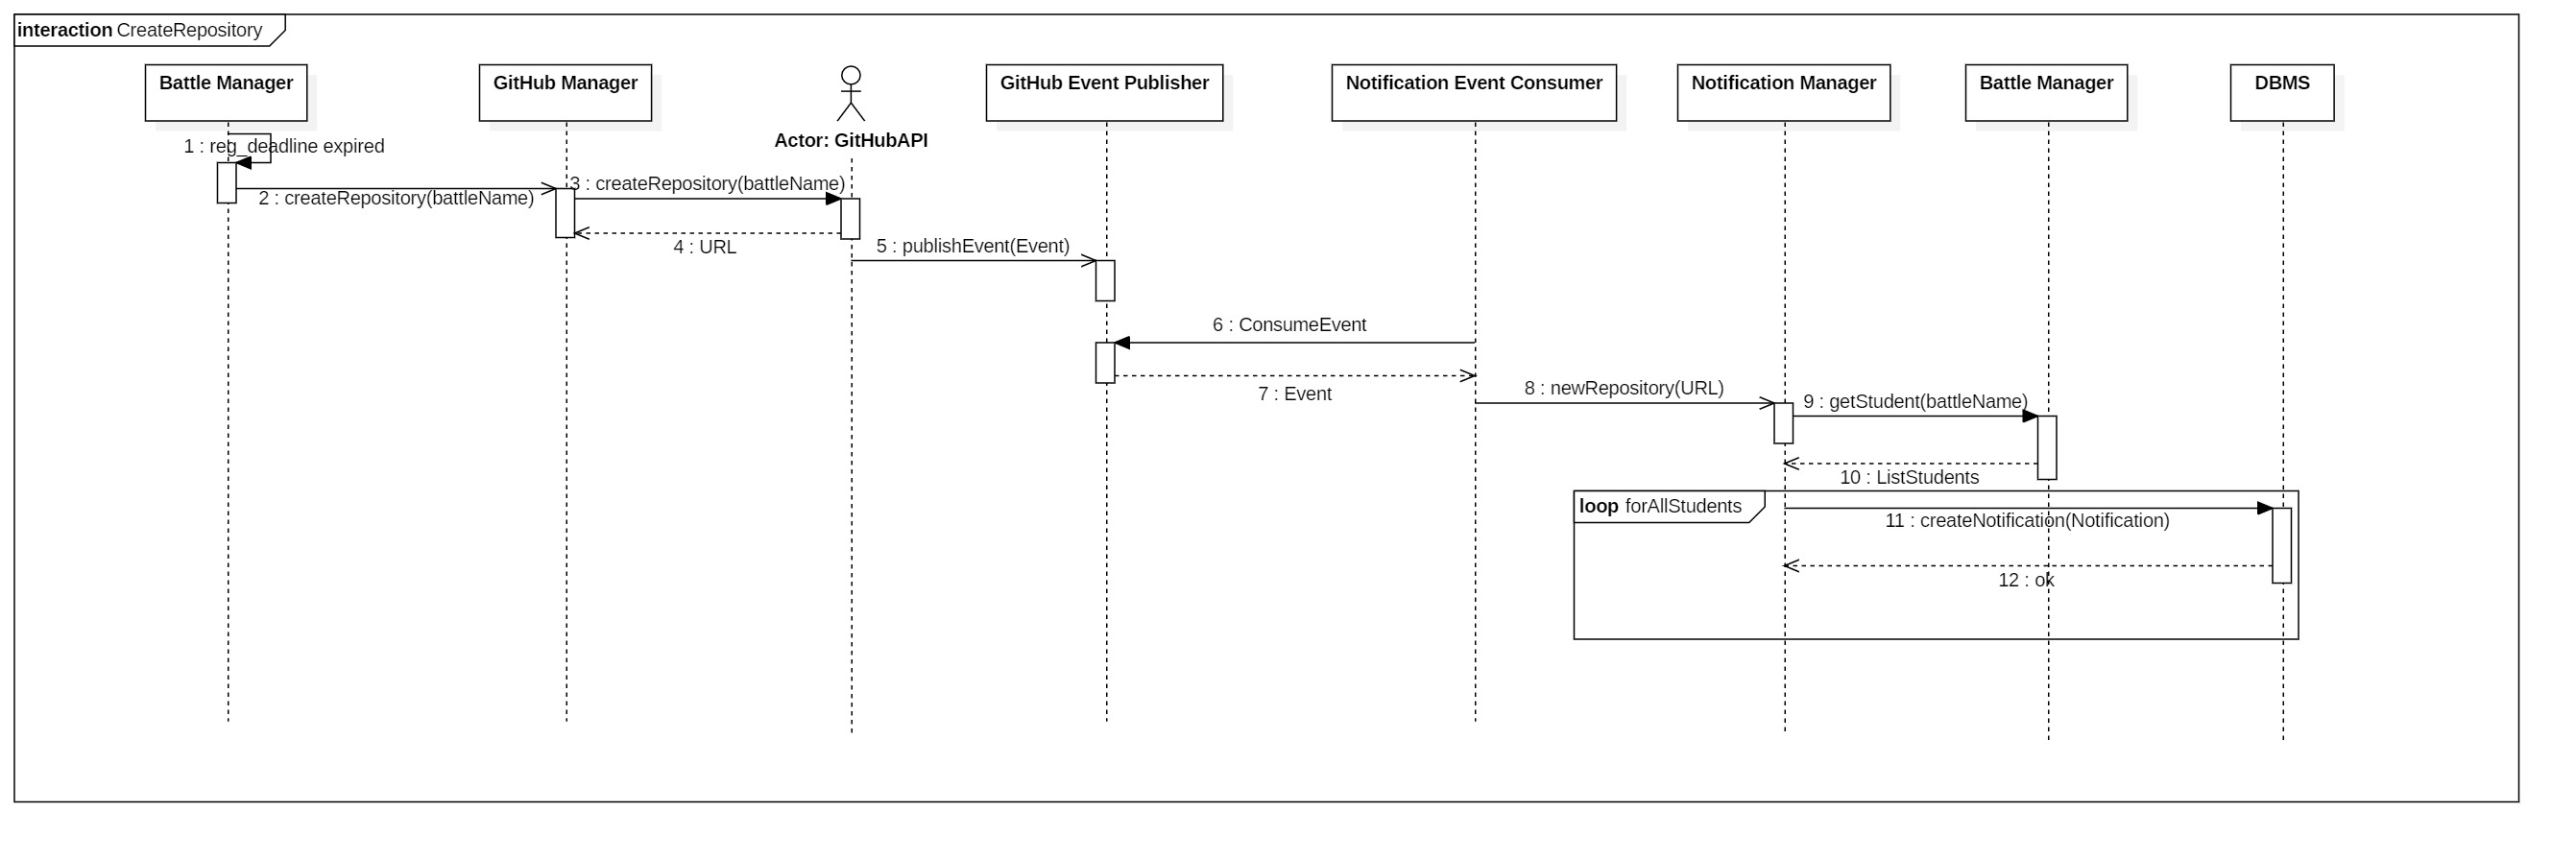
\includegraphics[width=1.3\linewidth, angle=90]{2.ArchitecturalDesign/res/CreateRepository.jpg}
    \caption{Runtime view for creating a repository}
    \label{fig:create_repo}
\end{figure}

The process begins when the Battle Manager detects that the registration deadline for a battle has expired. Following this event, the Battle Manager sends a request to the GitHub Manager to create a new repository for that battle. The GitHub Manager forwards this request to the GitHubAPI, which responds by providing the URL of the newly created repository.
Upon receiving this information, the GitHub Manager publishes a new Event for the Notification Consumer. Subsequently, the Notification Consumer sends notifications to all the students participating in that battle, creating them as described before.

\newpage


